\problemname{Pyramidbygge}

\begin{figure}[h!]
  \centering
  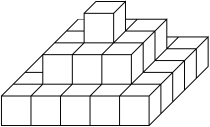
\includegraphics[scale=1.5]{pyramid}
\end{figure}

När man ska inleda ett större projekt, exempelvis bygga en pyramid, är det bäst att tänka efter en gång extra.
Du ska skriva ett program som beräknar hur hög pyramid man kan bygga om man har tillgång till ett visst antal stenblock.

Vi antar att pyramiden är kompakt, d.v.s. det finns inga hålrum inuti.
Vidare byggs den enligt principen i figuren ovan.
Varje lager är alltså kvadratiskt med en sidlängd som är två block mindre än det underliggande lagrets.
Det översta lagret består alltid av ett ensamt block.

Programmet ska fråga efter antalet tillgängliga block (högst hundra miljoner) och skriva ut höjden (i block räknat) för den största pyramid som kan byggas.
Det gör ingenting om det blir block över, men det får inte saknas ett enda block.

\section*{Indata}
Indata består av ett enda heltal: antal tillgängliga block.

\section*{Utdata}
Programmet ska skriva ut en rad med ett heltal: höjden för den största pyramid som kan byggas.
